\chapter{Angular}\label{funzionamento}

\section{Introduzione}

La pagina Angular mostra due differenti bottoni , uno di Fetch dello stato della API e un altro che modifica lo stato dell'entitá\footnote{nel dominio del POC, la prima entitá ID=1} , in questo bottone di modifica,il comportamento é quello di fetchare lo stato della lampada,per poi modificarlo nel suo complementare.
Vengono Dichiarati i componenti Angular "app" e "lamp-button" , che inglobano rispettivamente i fogli di stile e Markup , oltre che i rispettivi file typescript "component.ts" e ".module.ts" \footnote{per il componente app}. 
Vengono dichiarati i moduli "BrowserModule" , essenziale per lanciare una app browser, e "HttpClientModule" , essenziale per fare richieste HTTP,e' cosi' possibile implementare una GET , POST , DELETE oppure PUT. 
Nel Dominio del PoC si offrono tramite il metodo toggleLamp() , l'implementazione di una PUT per cambiare lo stato della lampada, innestato in una GET, capace di richiedere lo stato corrente della lampada stessa.

\subsection{getData\footnote{}}

Si offre il metodo getData\footnote{}, il quale da una chiamata GET all'url dello stato di tutte le lampade , quindi il loro id , il loro stato attuale \footnote{acceso = on , spento = off} e la loro locazione.

\subsection{toggleLamp\footnote{}}

Si offre il metodo toggleLamp(),tale metodo fa una chiamata "this.http.get<any>" su lamps/1 , si aspetta una risposta di tipo JSON e porta tale risposta alla richiesta innestata "this.http.put<any>" , la quale verifica lo stato del sotto campo dell'oggetto Response, Response.status, e lo cambia con il suo complementare \footnote{status: Response.status == 'on' ? 'off' : 'on'}.\\
Ritorna, alla fine della PUT, un Console.log con l'oggetto Response, che in questo momento temporale e' pari al risultato della operazione \footnote{e' stato fatto l'update , se modifica portata a buon fine}.

\begin{figure}[H]
    \centering
    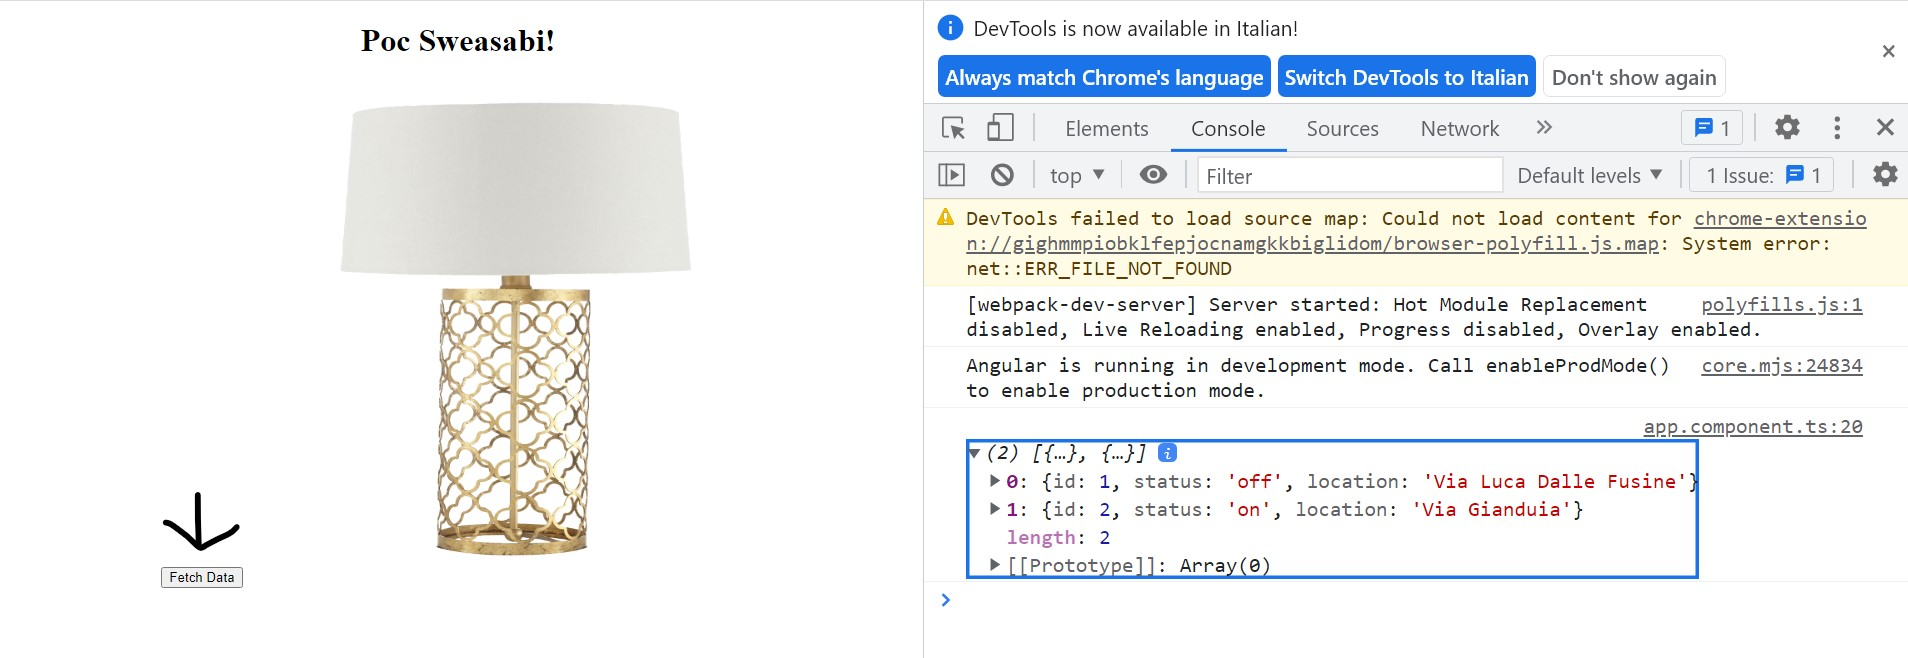
\includegraphics{getlamps.jpg}
    \caption{Button fa richiesta su /Lamps}
\end{figure}


\begin{figure}[H]
    \centering
    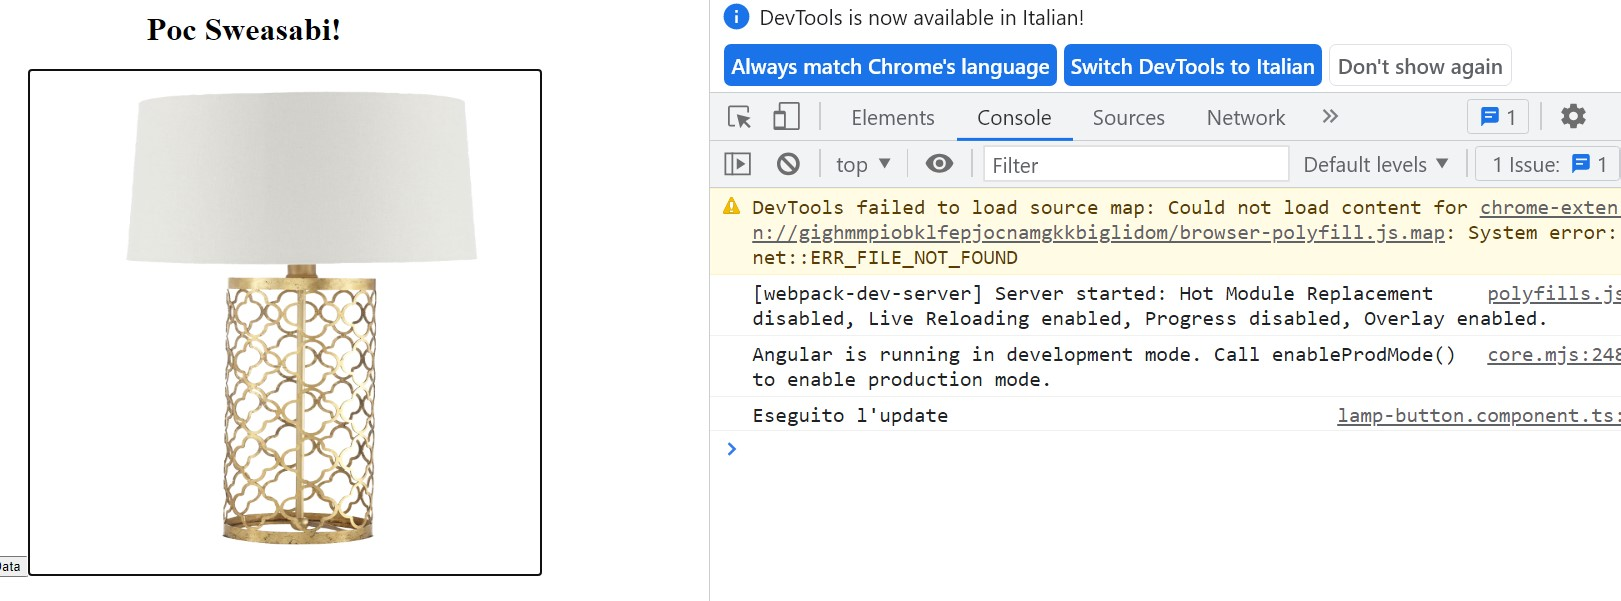
\includegraphics{modifylamps.jpg}
    \caption{Button fa cambio di stato su /Lamps/1}
\end{figure}

\begin{figure}[H]
    \centering
    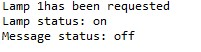
\includegraphics{modifylamps2.jpg}
    \caption{Button fa cambio di stato su /Lamps/1}
\end{figure}